\documentclass{article}
\usepackage{amsmath}
\usepackage[utf8]{inputenc}
\usepackage{graphicx}
\usepackage{verbatim}
\usepackage{float}
\usepackage[makeroom]{cancel}
\usepackage[english]{babel}
\usepackage{textcomp}
\usepackage{gensymb}
\usepackage{color}
\usepackage{subcaption}
\usepackage{caption}
\usepackage{hyperref}
\usepackage{physics}
\usepackage{dsfont}
%\usepackage{amsfonts}
\usepackage{listings}
\usepackage{multicol}
\usepackage{units}

% From Eirik's .tex
\usepackage{epstopdf}
\usepackage{cite}
\usepackage{braket}
\usepackage{url}
\bibliographystyle{plain}

\usepackage{algorithmicx}
\usepackage{algorithm}% http://ctan.org/pkg/algorithms
\usepackage{algpseudocode}% http://ctan.org/pkg/algorithmicx

\usepackage[margin=1cm]{caption}
\usepackage[outer=1.2in,inner=1.2in]{geometry}
% For writing full-size pages
%\usepackage{geometry}
%\geometry{
%  left=5mm,
%  right=5mm,
%  top=5mm,
%  bottom=5mm,
%  heightrounded,
%}

% Finding overfull \hbox
\overfullrule=2cm

\lstset{language=IDL}
 %\lstset{alsolanguage=c++}
\lstset{basicstyle=\ttfamily\small}
 %\lstset{backgroundcolor=\color{white}}
\lstset{frame=single}
\lstset{stringstyle=\ttfamily}
\lstset{keywordstyle=\color{red}\bfseries}
\lstset{commentstyle=\itshape\color{blue}}
\lstset{showspaces=false}
\lstset{showstringspaces=false}
\lstset{showtabs=false}
\lstset{breaklines}
\lstset{aboveskip=20pt,belowskip=20pt}

\lstset{basicstyle=\footnotesize, basewidth=0.5em}
\lstdefinestyle{cl}{frame=none,basicstyle=\ttfamily\small}
\lstdefinestyle{pr}{frame=single,basicstyle=\ttfamily\small}
\lstdefinestyle{prt}{frame=none,basicstyle=\ttfamily\small}
% \lstinputlisting[language=Python]{filename}


\definecolor{codepurple}{rgb}{0.58,0,0.82}
\definecolor{backcolour}{rgb}{0.95,0.95,0.92}
\definecolor{dkgreen}{rgb}{0,0.6,0}
\definecolor{gray}{rgb}{0.5,0.5,0.5}
\definecolor{magenta}{rgb}{0.58,0,0.82}

\lstdefinestyle{pystyle}{
  language=Python,
  aboveskip=3mm,
  belowskip=3mm,
  columns=flexible,
  basicstyle={\small\ttfamily},
  backgroundcolor=\color{backcolour},
  commentstyle=\color{dkgreen},
  keywordstyle=\color{magenta},
  numberstyle=\tiny\color{gray},
  stringstyle=\color{codepurple},
  basicstyle=\footnotesize,
  breakatwhitespace=false,
  breaklines=true,
  captionpos=b,
  keepspaces=true,
  numbers=left,
  numbersep=5pt,
  showspaces=false,
  showstringspaces=false,
  showtabs=false,
  tabsize=2
}

%%%%%%%%%%%%%%%%%%%%%%%%%%%%%%%%
% Self made macros here yaaaaaay
\newcommand\answer[1]{\underline{\underline{#1}}}
\newcommand\pd[2]{\frac{\partial #1}{\partial #2}}
\newcommand\red[1]{\textcolor{red}{\textbf{#1}}}
\newcommand\numberthis{\addtocounter{equation}{1}\tag{\theequation}}
% Usage: \numberthis \label{name}
% Referencing: \eqref{name}

% Some matrices
\newcommand\smat[1]{\big(\begin{smallmatrix}#1\end{smallmatrix}\big)}
\newcommand\ppmat[1]{\begin{pmatrix}#1\end{pmatrix}}

%%%%%%%%%%%%%%%%%%%%%%%%%%%%%%%%%
% Eirik's self made macros
\newcommand{\s}{^{*}}
\newcommand{\V}[1]{\mathbf{#1}}
\newcommand{\husk}[1]{\color{red} #1 \color{black}}
\newcommand{\E}[1]{\cdot 10^{#1}}
\newcommand{\e}[1]{\ \text{#1}}
\newcommand{\tom}[1]{\big( #1 \big)}
\newcommand{\Tom}[1]{\Big( #1 \Big)}
\newcommand{\tomH}[1]{\big[ #1 \big] }
\newcommand{\TomH}[1]{\Big[ #1 \Big]}
\newcommand{\tomK}[1]{ \{ #1 \} }
\newcommand{\TomK}[1]{\Big\lbrace #1 \Big\rbrace}
\newcommand{\bigabs}[1]{\left| #1 \right|}

% Section labeling
\usepackage{titlesec}% http://ctan.org/pkg/titlesec
\renewcommand{\thesubsection}{\arabic{subsection}}

% Title/name/date
\title{FYS4150 - Project 5\\$N$-body simulation of an open galactic cluster}
\author{Simen Nyhus Bastnes \& Eirik Ramsli Hauge}
\date{9. December 2016}

\begin{document}
\maketitle
\begin{abstract}
\begin{figure}[H]
\centering

\includegraphics[scale=0.5]{totoro.jpg}
\end{figure}
\end{abstract}
\subsection{Introduction}
In this project we will attempt to develop code that can be used for gravitational $N$-body simulations. Taking inspiration from an article by M. Joyce and co-workers \red{cite}, we will build a simple model of an open galactic cluster.
\\\\
An open cluster is a group consisting of up to a few thousand gravitationally bound stars, created from the collapse of a molecular cloud, and are usually found in the arms of spiral galaxies or in in irregular galaxies. The collapse of the cloud leads to a burst of star formation. As the stars of the cluster are of similar age and chemical composition, they are very import objects in the study of stellar evolution. Once formed, they gradually dissipate as members are ejected due to random interactions with other clusters, clouds of gas, or internal collisions.
\\\\
First, we look at some of the physics behind our model, making sure to find ideal units to fit our timescale. Running our model for $N = 100$ particles, we check the stability of our system, and find an ideal smoothing function for the gravitational force to remove some of the numerical instabilities. Having done that, we check how long the system takes to stabilize, conservation of energy, and checking the fraction of particles ejected from the system. Looking at only the bound particles, we can check if our results are consistent with the virial theorem.
\red{write motivation for why N body simulations}
\\\\
Finally, we increase the number of particles while keeping the total mass constant, to see how the radial density looks like. This can then be compared to well known profiles such as the Navarro-Frenk-White profile.

\subsection{Theory}

\subsubsection{N-body simulation}
In order to make our model of an open cluster, we will first look at some of the assumptions we make.
\begin{itemize}
  \item Consists of $N$ separate particles only interacting with each other via the Newtonian gravitational force. The force between two particles are then
    \begin{align*}
      F_G = -\frac{G M_1, M_2}{r^2}\numberthis\label{eq:newton}
    \end{align*}
    where $G$ is the gravitational constant, $r$ is the distance between the particles, and $M_1$, $M_2$ is the mass of the particles. For most of the project, we will be looking at $N=100$ particles.
  \item Since the only interaction is the gravitational force, the system is collisionless. If the probability of interactions between particles is low, then collisions have no significant effect on the results. For very large $N$, this might not hold as well.
  \item The particles start with little or no initial velocity, so-called \textit{cold collapse}.
  \item The particles are uniformly distributed within a sphere of radius $R_0 = 20$ ly. Masses are randomly distributed by a Gaussian distribution around $10\,M_{\odot}$ with a deviation of one solar mass.
\end{itemize}
Earlier this fall, we made a model of our solar system. \red{cite report 3} We recall that for a system only affected by Newtonian gravity, Newton's second law of motion gives us the following differential equations for particle $i$
\begin{align*}
  \frac{d^2\mathbf{r_i}}{dt^2} &= \sum\limits_{j\neq i}\frac{F_G(\mathbf{r}_{ij}, M_i,M_j)}{M_i}\numberthis\label{eq:diff_eq}
\end{align*}
where $\mathbf{r}$ is a three-dimensional vector in $(x,y,z)$, and we sum over the gravitational contribution of the other particles. We note that the length and timescale should be adjusted to units more fit for the dynamics of the system.\\\\
For the length scale, we can use lightyears, as the particles are initially uniformly distributed inside a sphere of radius $R_0 = 20$ ly. In order to find units of time that fit the timescale however, we will take a short detour into non-linear perturbation theory and cosmology.
% def metal():

\subsubsection{The spherical top-hat model}
While solving non-linear perturbation theory analytically can be difficult (or impossible), there does exists an analytical solution for the so-called ``\textit{spherical top-hat}'' model \red{cite cosmo notes}. In this model, we look at a spherical perturbation of radius $R$, with a uniform density inside. It can be shown that this model has a parametrised solution
\begin{align*}
  R &= A(1-\cos\theta)\numberthis\label{eq:top-hat}\\
  t &= B(\theta-\sin\theta)\\
  &A^3 = GMB^2 
\end{align*}
From equation \eqref{eq:top-hat}, we see that the sphere reaches a maximum at $\theta = \pi$, at time $t=\pi B$ (also referred to as turn-around). The sphere collapses completely at $\theta = 2\pi$, at time $t = 2\pi B$. At $\theta = \tfrac{3\pi}{2}$, the model virializes at radius $1/2 R_0$. For the peak radius
\begin{align*}
  R(\theta = \pi) &= 2A = R_0\\
  t(\theta = \pi) &= \pi B
\end{align*}
Solving for $B$
\begin{align*}
  B &= \frac{A^{3/2}}{\sqrt{GM}}
  \intertext{Using that the density of the perturbation is given by $\rho_0 = M/V = M/(4/3\pi R_0^3)$}
  B &= \frac{(R_0/2)^{3/2}}{\sqrt{G\frac{4\pi R_0^3\rho_0}{3}}}\\
  B &= \sqrt{\frac{3}{32\pi G\rho_0}}
\end{align*}
Since our simulation starts with cold collapse (at turn-around $\theta = \pi$), the time it takes to collapse is
\begin{align*}
  t_{\text{coll}} &= t_{2\pi} - t_{\pi}\\
  t_{\text{coll}} &= 2\pi B - \pi B = \pi B
  \intertext{inserting the expression we found for $B$, we get the collapse time}
  t_{\text{coll}} &= \sqrt{\frac{3\pi}{32G\rho_0}}\numberthis\label{eq:t_coll}
\end{align*}
As this time, $t_{\text{coll}}$ is an analytical expression for collapse in the \textit{spherical top-hat model}, this is a much more fitting timescale to probe our system with compared to seconds or years.\\\\
In order to make use of this, we need to scale equation \eqref{eq:newton} in these units, specifically $G$. Rewriting equation \eqref{eq:t_coll} gives us
\begin{align*}
  G &= \frac{3\pi}{32\rho_0t_{\text{coll}}^2}
  \intertext{Scaling so that we are looking at timescales of order $t_{\text{coll}}$, and inserting $\rho_0 = 4/3\pi R_0^3$}
  G &= \frac{\pi^2R_0^3}{8M_{tot}} = \frac{\pi^2R_0^3}{8N\mu} \numberthis\label{eq:G}
\end{align*}
where $N$ is the number of particles, and $\mu$ is the average mass (in solar masses) per particle.\\\\
Inserting equation \eqref{eq:G} into the differential equation given by \eqref{eq:diff_eq} gives us the units $[\text{ly}/t_{\text{coll}}]$, which is what we wanted.
%Page 18ish in cosmo1.5 lecture notes\\
%collapse time, spherical top hat model, virialization.
%Sphere completely collapses at $\theta = 2\pi$ \red{add image maybe?}

\subsubsection{Numerical instabilities}
Since we will be solving the system numerically, we have to be aware of some of the problems of doing so. In this project, we will focus on the numerical instability that arises when two particles come very close to each other. When two particles get close to each other, the accelerations get large, and unless we have very small timesteps, the trajectory of a particle is not calculated accurately. To deal with this, we will introduce a very simple smoothing function by modifying the Newtonian force \eqref{eq:newton}
\begin{align*}
  F_{\text{mod}} &= \frac{GM_1M_2}{r^2 + \varepsilon^2} \numberthis\label{eq:newton_mod}
\end{align*}
where $\varepsilon$ is a small real constant that causes equation \eqref{eq:newton_mod} to be finite on short length scales. While adding this smoothing factor smoothes out the instabilities, it also means that on length scales smaller than $\varepsilon$, the trajectories are not integrated accurately. This means that we should make sure to set the smoothing factor $\varepsilon$ to a length so that 1) instabilities are smoothed out, and 2) the inaccuracy in the trajectory does not play a significant part of the macroscopic evolution of the system.\\\\
As we discussed earlier, we assume the system to be collisionless, and that collisions (or close encounters) should not affect the system much. Since our particles does not represent point particles, but mass distributions with some finite radius, a really close encounter between two particles might not be fully collisionless. The smoothing factor does then in a sense represent the fact that our system is not fully collisionless, but the magnitude of it is most likely considerably larger than the scale at which collisions become relevant.\\\\
Finding an ideal size for $\varepsilon$ can be difficult. A simple way to evaluate this is to first find the mean interparticle distance. \red{cite Joyce full}
\begin{align*}
  l &\equiv \bigg(\frac{3V}{4\pi N}\bigg)^{1/3} = \frac{R_0}{N^{1/3}} \numberthis\label{eq:mean_dist}
\end{align*}
where $R_0$ is the initial radius of the sphere, and $N$ is the number of particles. Since this is the average distance between the particles at the start of the simulation, we should make sure that our choice of $\varepsilon$ is significantly less than $l$, as it limits how small the structure is allowed to collapse. For example, for the situation $R_0 = 20$ and $N = 100$, we have $l \approx 4.3$.

%try to find fitting size order from mean particle distance and refer to article
\subsubsection{Particle ejection}
Due to looking at a \textit{cold collapse}, all particles start with a negative energy, but as the system evolves, some of the particles can end up with a positive energy, and completely escape from the system. We can therefore identify these ejected particles by comparing the per particle kinetic and potential energy, and identifying which particles have a total energy greater than zero
\begin{align*}
  E_{i,\text{tot}} = K_i + V_i > 0 \numberthis\label{eq:ejection}
\end{align*}
where $K_i$ and $V_i$ is the kinetic and potential energy for particle $i$.\\\\
The energy taken away from the system by particle ejection can be found by energy conservation and that once the system stabilizes, the potential energy of the ejected particles and the interaction between bound and ejected particles is negligible
\begin{align*}
  E_0 &= V_b + K_b + K_f \numberthis\label{eq:energy_ejection}
\end{align*}
where $E_0$ is the initial energy of the system, $V_b$ and $K_b$ is the kinetic and potential energy of the particles that are gravitationally bound, and $K_f$ is the kinetic energy of the ejected particles.
$K_f$ can be found as discussed earlier in equation \eqref{eq:ejection}.

\subsubsection{Virial theorem}
For a bound gravitational system in equilibrium, the virial theorem says that
\begin{align*}
  2\langle K\rangle &= -\langle V\rangle \numberthis\label{eq:virial}
\end{align*}
where $\langle K\rangle$ is the time-average kinetic energy of the system, and $\langle V\rangle$ is the time-average potential energy. By the ergodic hypothesis, we can assume that an average over a large enough system should give the same result as the time average. Thus we have
\begin{align*}
  2K_b &= -V_b \numberthis\label{eq:virial2}
\end{align*}
where $K_b$ and $V_b$ are the energies for the bound particles, and can be found from equation \eqref{eq:energy_ejection}

\subsubsection{Radial density of particles}
For an approximately spherical symmetric collapsed halo (virialized structure), the radial density profile can often be fit very well with the simple expression
\begin{align*}
  n(r) = \frac{n_0}{\Big(1+(\frac{r}{r_0})^4\Big)} \numberthis\label{eq:radial_dist}
\end{align*}
where $n_0$ and the scale radius $r_0$ has some dependency on the number of particles $N$.\\\\
The well-known Navarro-Frenk-White profile can also be used to compare with results.
\begin{align*}
  \rho(r) &= \frac{\rho_0}{\frac{r}{r_0}\Big(1+\frac{r}{r_0}\Big)^2}\numberthis\label{eq:NFW}
\end{align*}
where $\rho_0$ and $r_0$ depends on $N$ in some way.
\subsubsection{Numerical solving}
In order to solve the system numerically, we will employ the Velocity Verlet method. A full derivation of the Velocity Verlet method can be found in \red{cite project 3}, where the following algorithm is also found.
\begin{algorithm}[H]
\small
\caption{Velocity Verlet}\label{alg:VelVerlet}
\begin{algorithmic}[1]
\For{$i = 0, n$}
\State $r_{i+1} = r_i + v_i h + \frac{1}{2} a_i h^2$
\State $a_{i+1} = F_{G, r_{i+1}}/m$
\State $v_{i+1} = v_i + \frac{1}{2} h (a_i + a_{i+1})$
\EndFor
\end{algorithmic}
\end{algorithm}
\subsection{Experimental}
The programs used in this project can be found in the GitHub repository \cite{GitHub}, in the \texttt{/src/} folder. When running the program it takes 4 command line arguments: \texttt{N}, \texttt{t\_coll}, \texttt{dt} and \texttt{eps}. \texttt{N} is the number of stars in our cluster, \texttt{t\_coll} is our time unit, based on the collision time, \texttt{dt} is the time step and \texttt{eps} is the smoothing factor used in the force calculation. All data written to file by the main program are stored in \texttt{/benchmarks/} where most of the data analysis were done by python programs stored in \texttt{/python/} and the figures and gifs can be found in \texttt{/figures/}. \\ \\
The simulation starts by randomly positioning different stars inside a sphere with radius R = 20 light years. Each star will have an individual mass where the total mass is forced to be 1000 solar masses and an initial velocity set to be 0 in all directions. \\
Once all the positions and masses have been set, we can find the forces acting between them. While using velocity verlet to simulate the behaviour we can also find the individual kinetic and potential energy of each star as well as the total kinetic and potential energy of the system. 
\subsection{Results}
%%%%%%%%%%%%%%%%%%%%%%%%%%%%%
%%%         task b        %%%
%%%%%%%%%%%%%%%%%%%%%%%%%%%%%
A simulation for N = 100 particles over a time of 5 collision times with a time step of 0.001 and no smoothing factor is plotted in figure \ref{fig:noepsmuchtime} for different times during the simulation. From these figures and the figure \ref{fig:noeps} we can see that without a smoothing factor we will never reach an equilibrium.
\begin{figure}[H]
\centering
\begin{subfigure}{0.49\textwidth}
	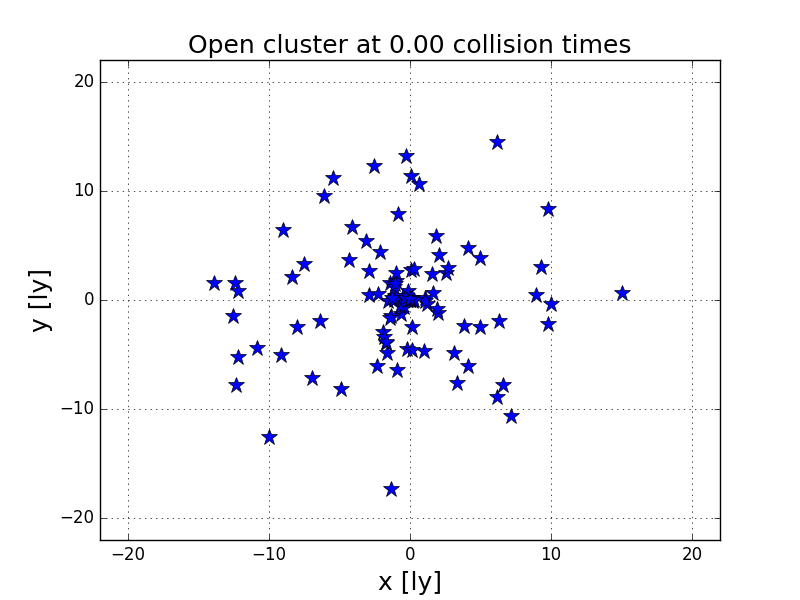
\includegraphics[scale=0.33]{{../figures/taskb/N100/plot_N100_time0.00}.png}
	\caption{At time 0.00 collision times}
	\label{subfig:noepsmuchtime1}
\end{subfigure}
\begin{subfigure}{0.49\textwidth}
	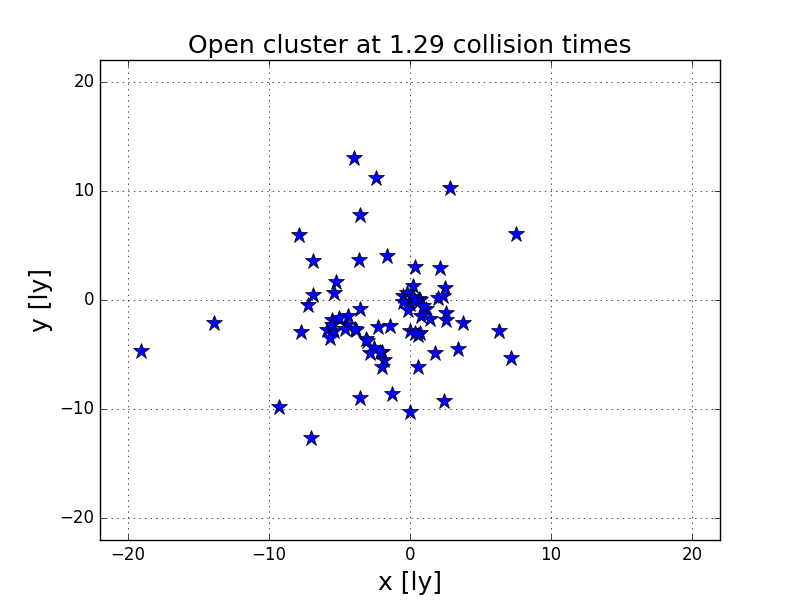
\includegraphics[scale=0.33]{{../figures/taskb/N100/plot_N100_time26.00}.png}
	\caption{At time 1.29 collision times}
	\label{subfig:noepsmuchtime2}
\end{subfigure}
\qquad
\begin{subfigure}{0.49\textwidth}
	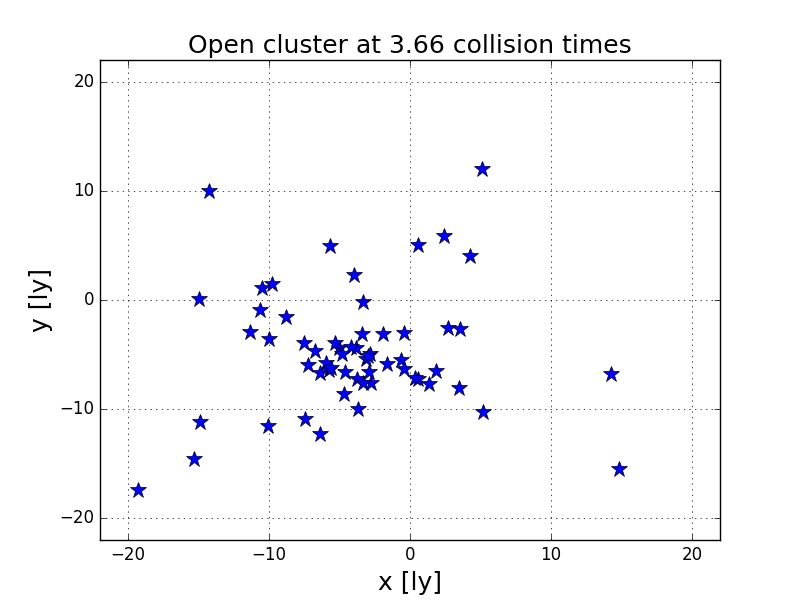
\includegraphics[scale=0.33]{{../figures/taskb/N100/plot_N100_time74.00}.png}
	\caption{At time 3.66 collision times}
	\label{subfig:noepsmuchtime3}
\end{subfigure}
\begin{subfigure}{0.49\textwidth}
	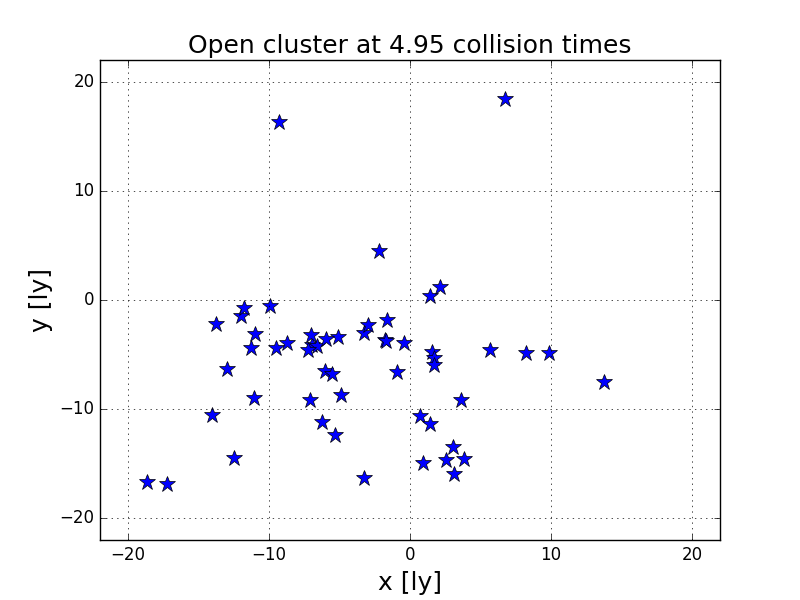
\includegraphics[scale=0.33]{{../figures/taskb/N100/plot_N100_time100.00}.png}
	\caption{At time 4.95 collision times}
	\label{subfig:noepsmuchtime4}
\end{subfigure}
\caption{Position of each star in 2D as a function of time.}
\label{fig:noepsmuchtime}
\end{figure}
%%%%%%%%%%%%%%%%%%%%%%%%%%%%%
%%%         task c        %%%
%%%%%%%%%%%%%%%%%%%%%%%%%%%%%
Letting our program run for different number of particles we found the total energy, the fraction of particles with positive total energy and the kinetic energy of the escaped particles. These results are shown below in figure \ref{fig:noeps}.

\begin{figure}[H]
\centering
\begin{subfigure}{0.49\textwidth}
	\includegraphics[scale=0.33]{{../figures/taskc/totenergy_N100}.png}
	\caption{Number of particles: 100}
	\label{subfig:noeps100}
\end{subfigure}
\begin{subfigure}{0.49\textwidth}
	\includegraphics[scale=0.33]{{../figures/taskc/totenergy_N200}.png}
	\caption{Number of particles: 200}
	\label{subfig:noeps200}
\end{subfigure}
\qquad
\begin{subfigure}{0.49\textwidth}
	\includegraphics[scale=0.33]{{../figures/taskc/totenergy_N500}.png}
	\caption{Number of particles: 500}
	\label{subfig:noeps500}
\end{subfigure}
\begin{subfigure}{0.49\textwidth}
	\includegraphics[scale=0.33]{{../figures/taskc/totenergy_N1000}.png}
	\caption{Number of particles: 1000}
	\label{subfig:noeps1000}
\end{subfigure}
\caption{Total energy and fraction of particles with positive total energy for different number of particles without a smoothing factor.}
\label{fig:noeps}
\end{figure}
%%%%%%%%%%%%%%%%%%%%%%%%%%%%%
%%%         task d        %%%
%%%%%%%%%%%%%%%%%%%%%%%%%%%%%
To find the best smoothing factor discussed above in the theory we used the trial and error method. For 200 stars with a time step of 0.001 and a time from 0 to 5 collision times we found the total energy as presented in figure \husk{fig:totalEnergy}
\begin{figure}[H]
\centering
\begin{subfigure}{0.49\textwidth}
	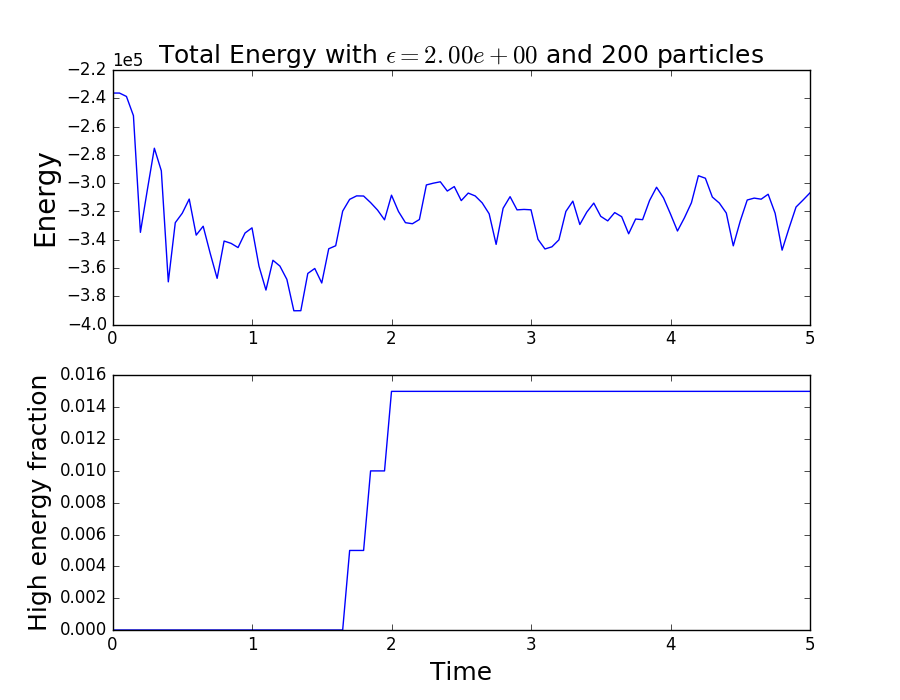
\includegraphics[scale=0.33]{{../figures/taskd/totenergy_eps2.00e+00_N200}.png}
	\caption{$\epsilon$ = 2.0}
	\label{subfig:eps2}
\end{subfigure}
\qquad
\begin{subfigure}{0.49\textwidth}
	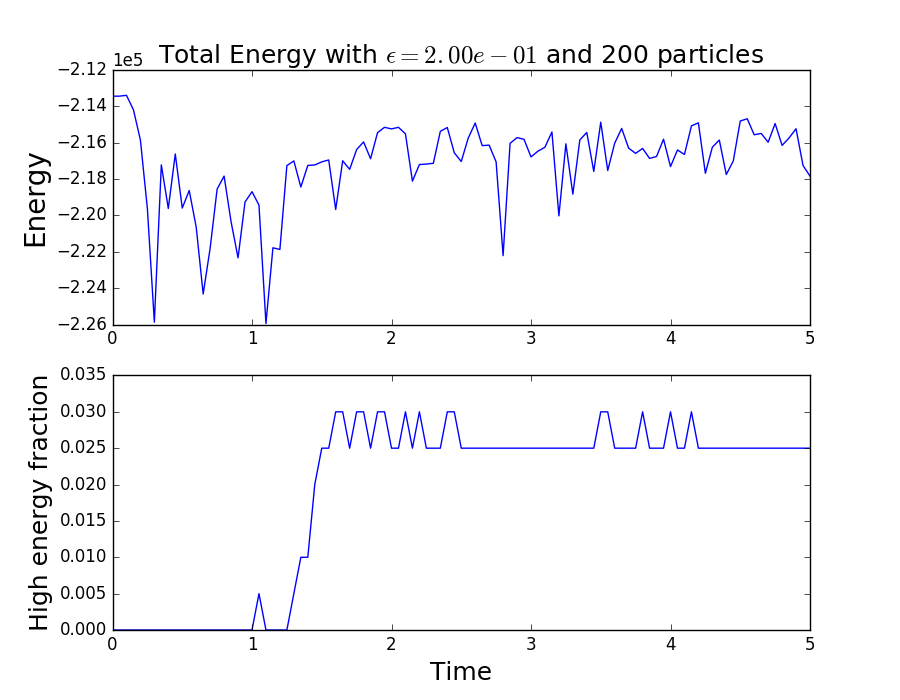
\includegraphics[scale=0.33]{{../figures/taskd/totenergy_eps2.00e-01_N200}.png}
	\caption{$\epsilon$ = 0.2}
	\label{subfig:eps0.2}
\end{subfigure}
\begin{subfigure}{0.49\textwidth}
	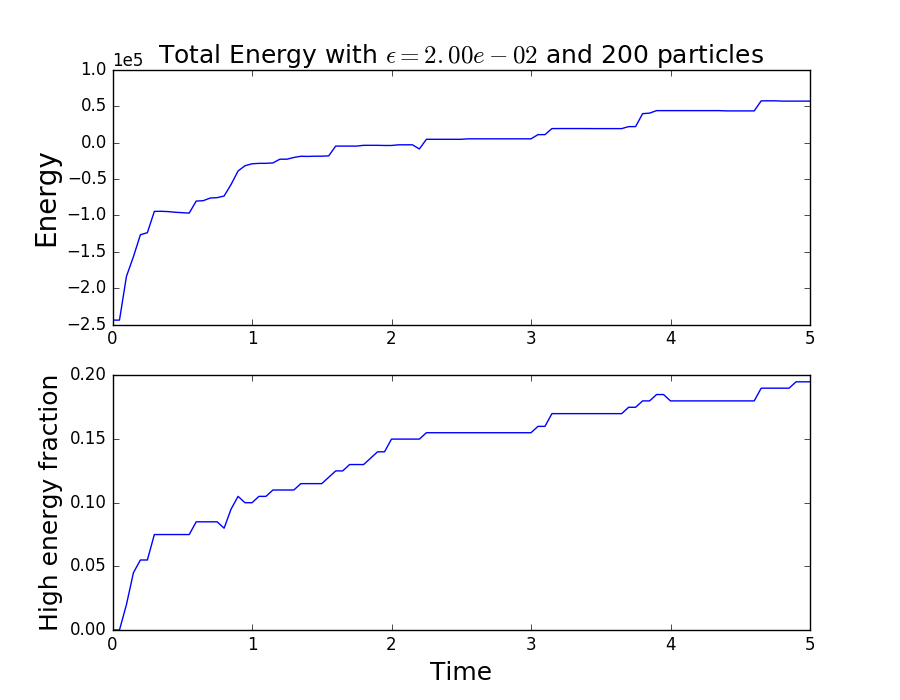
\includegraphics[scale=0.33]{{../figures/taskd/totenergy_eps2.00e-02_N200}.png}
	\caption{$\epsilon$ = 0.02}
	\label{subfig:eps0.02}
\end{subfigure}
\caption{Total energy and fraction of particles with positive total energy for different smoothing factors for a simulation of 200 stars.}
\label{fig:totalEnergy}
\end{figure}
As we now have found a better smoothing factor we can once again simulate for different number of particles and see the difference. By setting a smoothing factor of 0.1 and simulating for different number of particles with time step 0.001 and over a time period of 5 collisions times the graphs in figure \ref{fig:eps}:
\begin{figure}[H]
\centering
\begin{subfigure}{0.49\textwidth}
	\includegraphics[scale=0.33]{{../figures/taskd/totenergy_N100}.png}
	\caption{Number of particles: 100}
	\label{subfig:noeps100}
\end{subfigure}
\begin{subfigure}{0.49\textwidth}
	\includegraphics[scale=0.33]{{../figures/taskd/totenergy_N200}.png}
	\caption{Number of particles: 200}
	\label{subfig:noeps200}
\end{subfigure}
\qquad
\begin{subfigure}{0.49\textwidth}
	\includegraphics[scale=0.33]{{../figures/taskd/totenergy_N500}.png}
	\caption{Number of particles: 500}
	\label{subfig:noeps500}
\end{subfigure}
\begin{subfigure}{0.49\textwidth}
	\includegraphics[scale=0.33]{{../figures/taskd/totenergy_N1000}.png}
	\caption{Number of particles: 1000}
	\label{subfig:noeps1000}
\end{subfigure}
\caption{Total energy and fraction of particles with positive total energy for different number of particles with a smoothing factor.}
\label{fig:noeps}
\end{figure}
%%%%%%%%%%%%%%%%%%%%%%%%%%%%%
%%%         task e        %%%
%%%%%%%%%%%%%%%%%%%%%%%%%%%%%
To see if we our results were consisten with the viral theorem, we checked if the average of the potential energy subtracted from two times the average of the bound particles kinetic energy  was zero. The result are plotted in figure \ref{fig:viral}
\begin{figure}[H]
\centering
\begin{subfigure}{0.49\textwidth}
	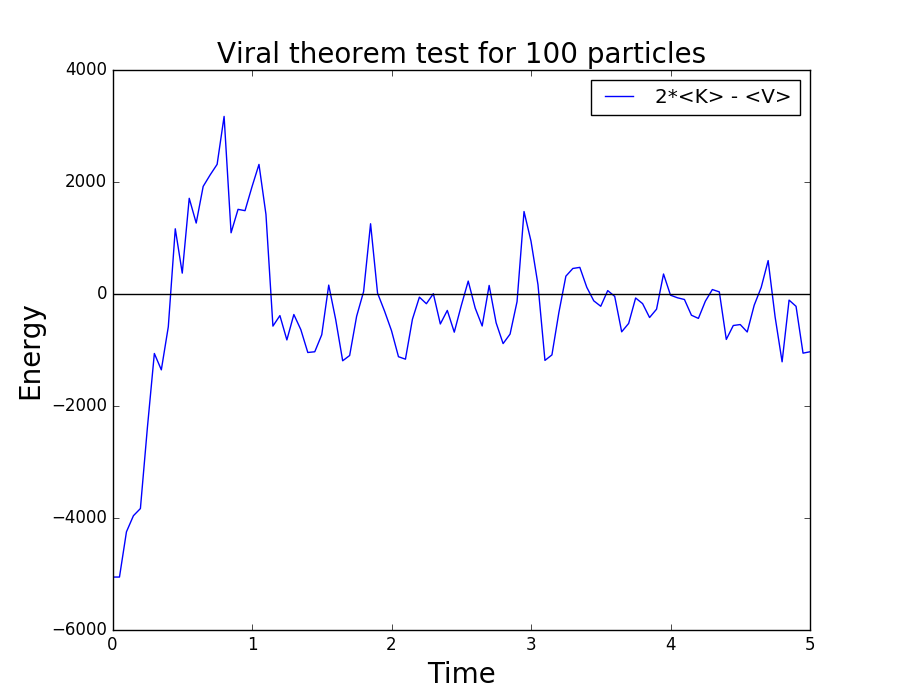
\includegraphics[scale=0.33]{{../figures/taske/viral_N100}.png}
	\caption{Number of particles: 100}
	\label{subfig:viral100}
\end{subfigure}
\qquad
\begin{subfigure}{0.49\textwidth}
	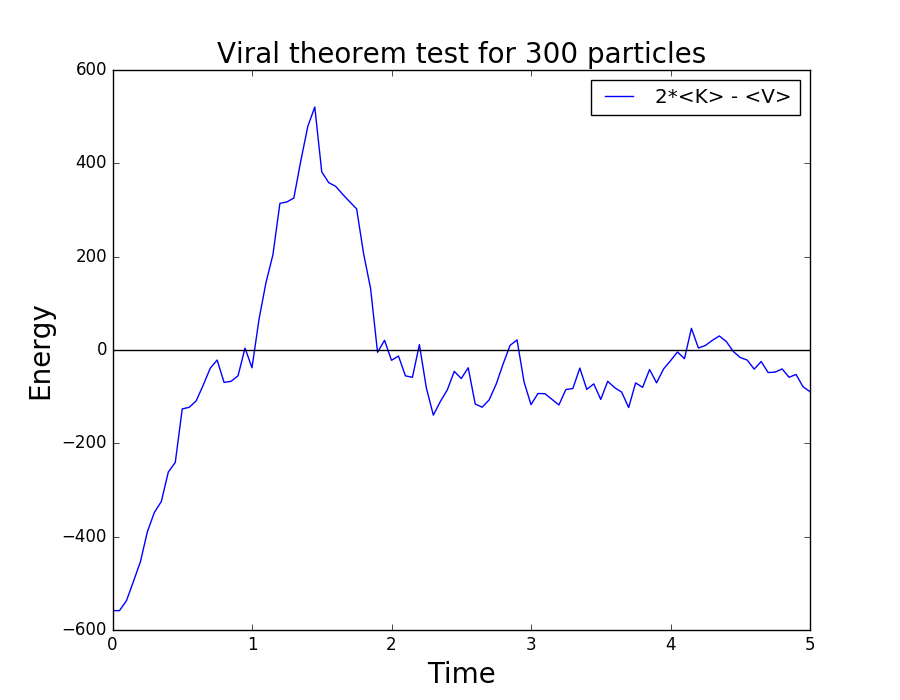
\includegraphics[scale=0.33]{{../figures/taske/viral_N300}.png}
	\caption{Number of particles: 300}
	\label{subfig:viral300}
\end{subfigure}
\begin{subfigure}{0.49\textwidth}
	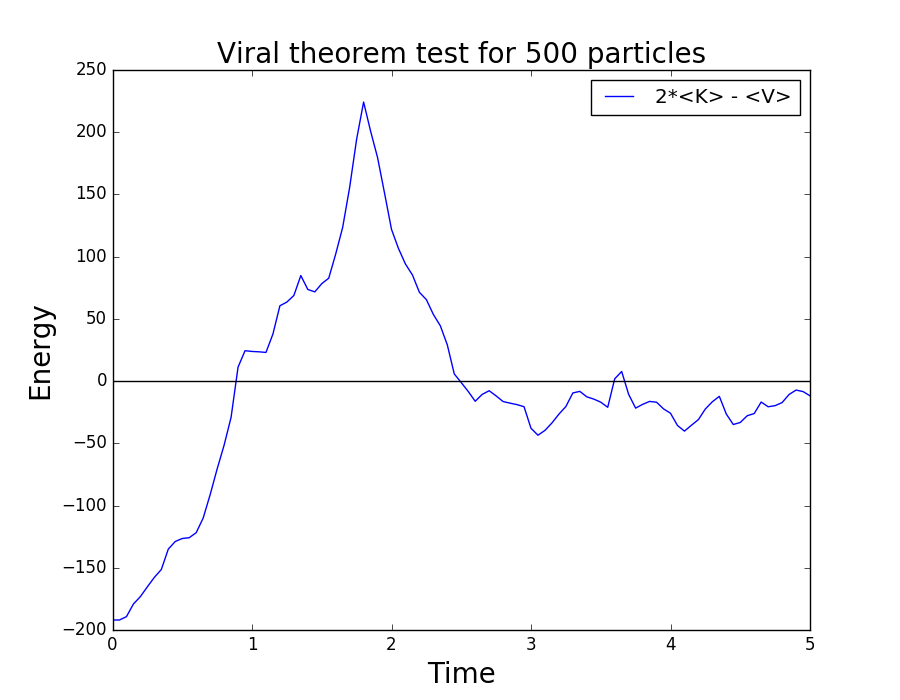
\includegraphics[scale=0.33]{{../figures/taske/viral_N500}.png}
	\caption{Number of particles: 500}
	\label{subfig:viral500}
\end{subfigure}
\caption{Total energy for different smoothing factors for a simulation of 200 stars.}
\label{fig:viral}
\end{figure}
%%%%%%%%%%%%%%%%%%%%%%%%%%%%%
%%%         task f        %%%
%%%%%%%%%%%%%%%%%%%%%%%%%%%%%
By simulating different number of particles with the same total mass we were able to find the radial density, mean distance from origo and the standard derivation of distance from origo (see figure \ref{fig:radialDens} and \ref{fig:meanstd})
\begin{figure}[H]
\centering
\begin{subfigure}{0.49\textwidth}
	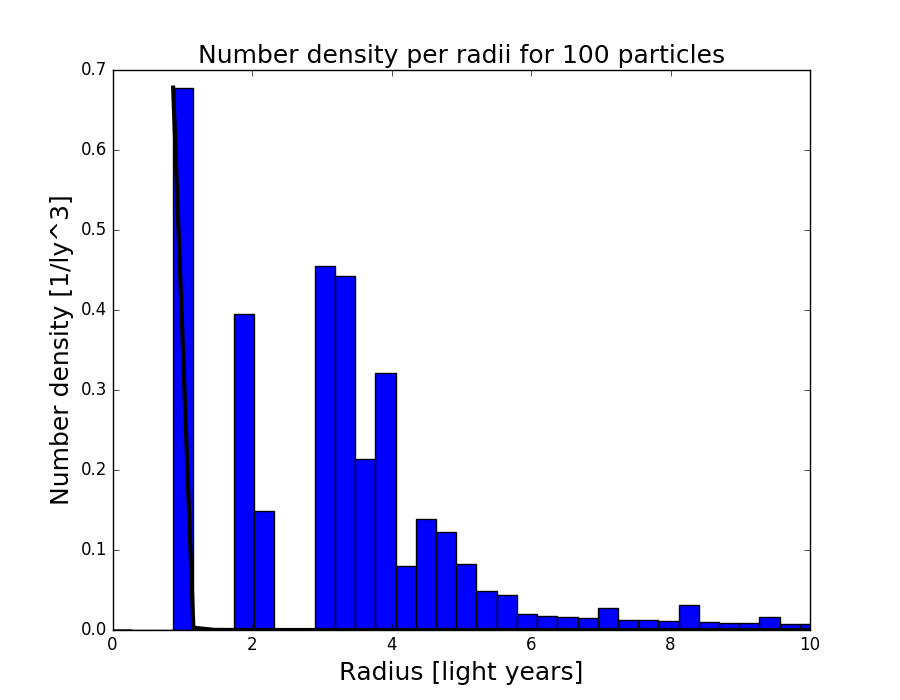
\includegraphics[scale=0.33]{{../figures/taskf/radialDens_N100}.png}
	\caption{Number of particles: 100}
	\label{subfig:radialDens100}
\end{subfigure}
\qquad
\begin{subfigure}{0.49\textwidth}
	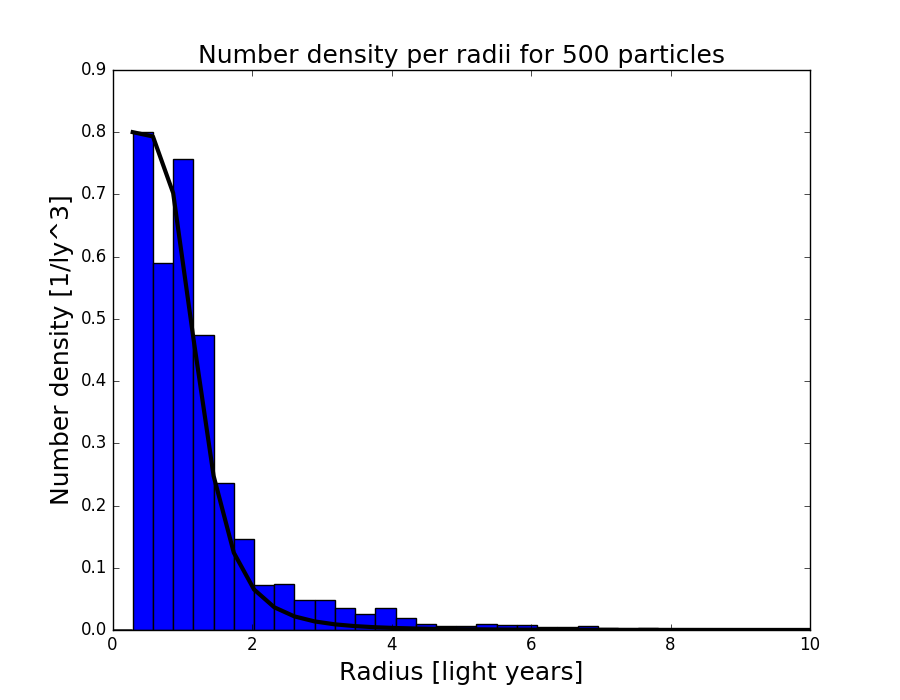
\includegraphics[scale=0.33]{{../figures/taskf/radialDens_N500}.png}
	\caption{Number of particles: 500}
	\label{subfig:radialDens500}
\end{subfigure}
\begin{subfigure}{0.49\textwidth}
	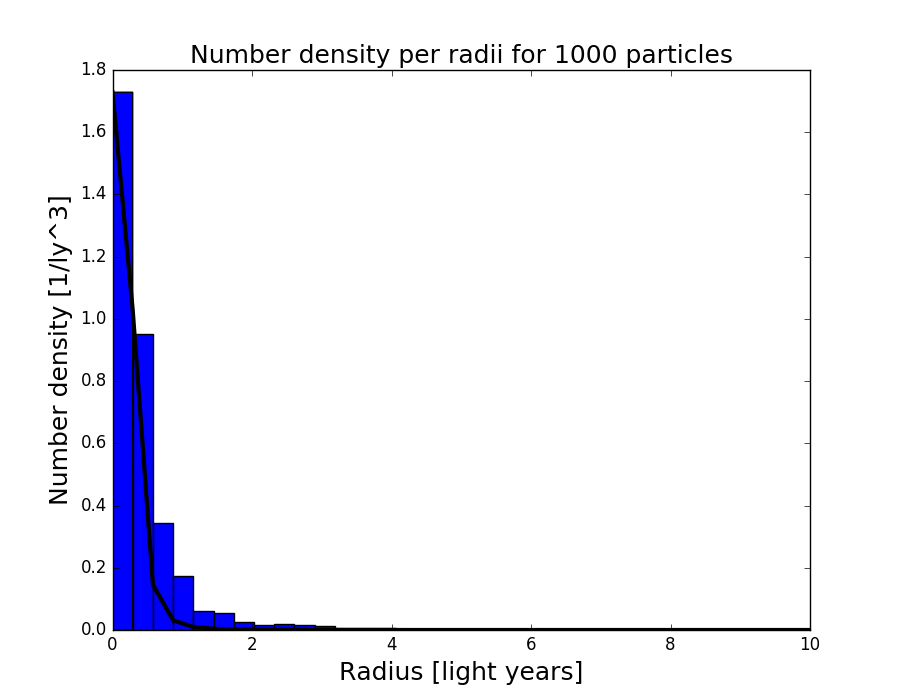
\includegraphics[scale=0.33]{{../figures/taskf/radialDens_N1000}.png}
	\caption{Number of particles: 1000}
	\label{subfig:radialDens1000}
\end{subfigure}
\caption{Radial density for different number of particles.}
\label{fig:radialDens}
\end{figure}
\begin{figure}[H]
\centering
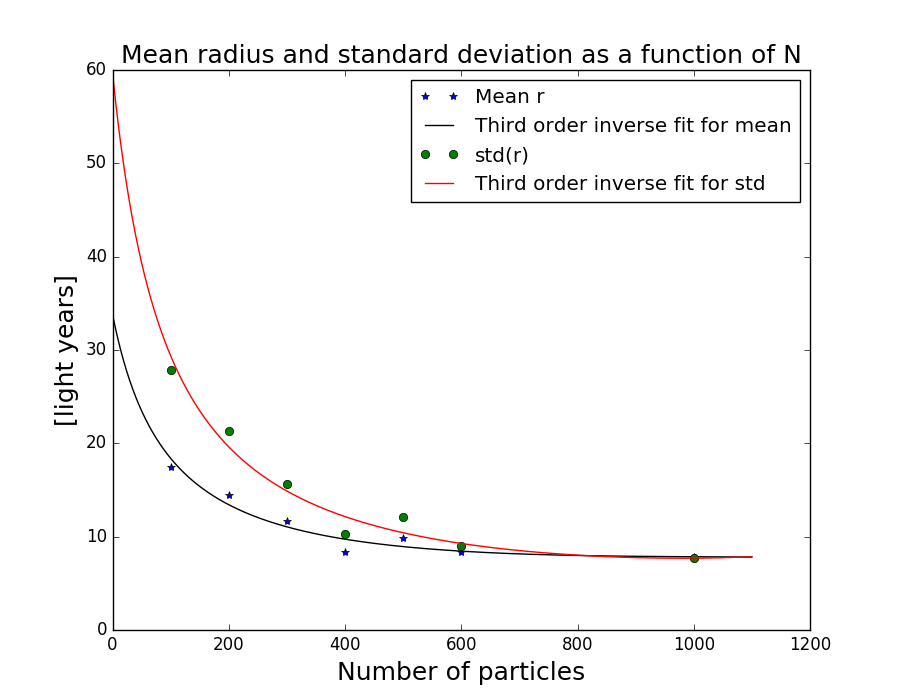
\includegraphics[scale=0.5]{{../figures/taskf/meanstd}.png}
\caption{Standard deviation and average distance from origo for all particles}
\label{fig:meanstd}
\end{figure}
\subsection{Discussion}
%%%%%%%%%%%%%%%%%%%%%%%%%%%%%
%%%         task a        %%%
%%%%%%%%%%%%%%%%%%%%%%%%%%%%%

%%%%%%%%%%%%%%%%%%%%%%%%%%%%%
%%%         task b        %%%
%%%%%%%%%%%%%%%%%%%%%%%%%%%%%

%%%%%%%%%%%%%%%%%%%%%%%%%%%%%
%%%         task c        %%%
%%%%%%%%%%%%%%%%%%%%%%%%%%%%%

%%%%%%%%%%%%%%%%%%%%%%%%%%%%%
%%%         task d        %%%
%%%%%%%%%%%%%%%%%%%%%%%%%%%%%

%%%%%%%%%%%%%%%%%%%%%%%%%%%%%
%%%         task e        %%%
%%%%%%%%%%%%%%%%%%%%%%%%%%%%%

%%%%%%%%%%%%%%%%%%%%%%%%%%%%%
%%%         task f        %%%
%%%%%%%%%%%%%%%%%%%%%%%%%%%%%
As we can see from figure \ref{fig:radialDens} the cluster is densest near origo. This is as expected 

\subsection{Conclusion}
\bibliography{references}
\end{document}
